\section{Verlustbehaftete Kompression von volumetrischen Punkten}
In verschiedene wissenschaftliche Simulationen wie Sonnenforschung, Magnetismus, Teilchenphysik, Quantenmechanik etc. produzieren grosse Datenmengen. Man möchte SChwingungen, Flugbahnen, Kraftfelder etc als Linien im dreidimensionalen Raum darstellen. Jede Linie besteht aus einer grossen Menge an volumetrischen Punkten.\\
In dieser Arbeit soll mit einer verlustbehafteten Kompression möglich gemacht werden, die Datenmenge über eine Internetverbindung zu übertragen. 

Computersimulationen produzieren grosse Datenmengen. 
In dieser Arbeit soll eineLinien, welche als Menge von volumetrischen Punkten abgebildet ist, verlustbehaftet komprimiert werden. sodass eine Übertragung über eine Internetverbindung in sinnvoller Zeit abgeschlossen ist. Die Artefakte der Kompression sollen sich im Rahmen halten. Aber dennoch schön aussehen.\\
[\baselineskip]
teilchenphysik, sonnenForschung, feldlinien Konkreter Anwendungsfall der JHelioviewer. Visualisiert Satellitenmessungen und Simulationen. Mittels PFSS werden die Feldlinien simuliert. Datenmenge soll nun auf den jeweiligen JHelioviewer des Sonnenforschers übertragen werden. (Feldlinienbild). Resultate\\
[\baselineskip]
Der JHelioviewer ist eine Applikation, die zur Analyse von Sonnendaten verwendet wird. Es wird international zur Sonnenforschung eingesetzt und wird von der FHNW zusammen mit der ESA entwickelt. Momentan ist eine neue Version des JHelioviewer in Entwicklung, welche die Sonne im dreidimensionalen Raum darstellt. Ein Feature von JHelioviewer ist die Magnetfeldlinien darzustellen und zu animieren, die Abbildung \ref{einleitung::feldlinien} zeigt die Visualisierung.
\begin{figure}[!htbp]
\center
	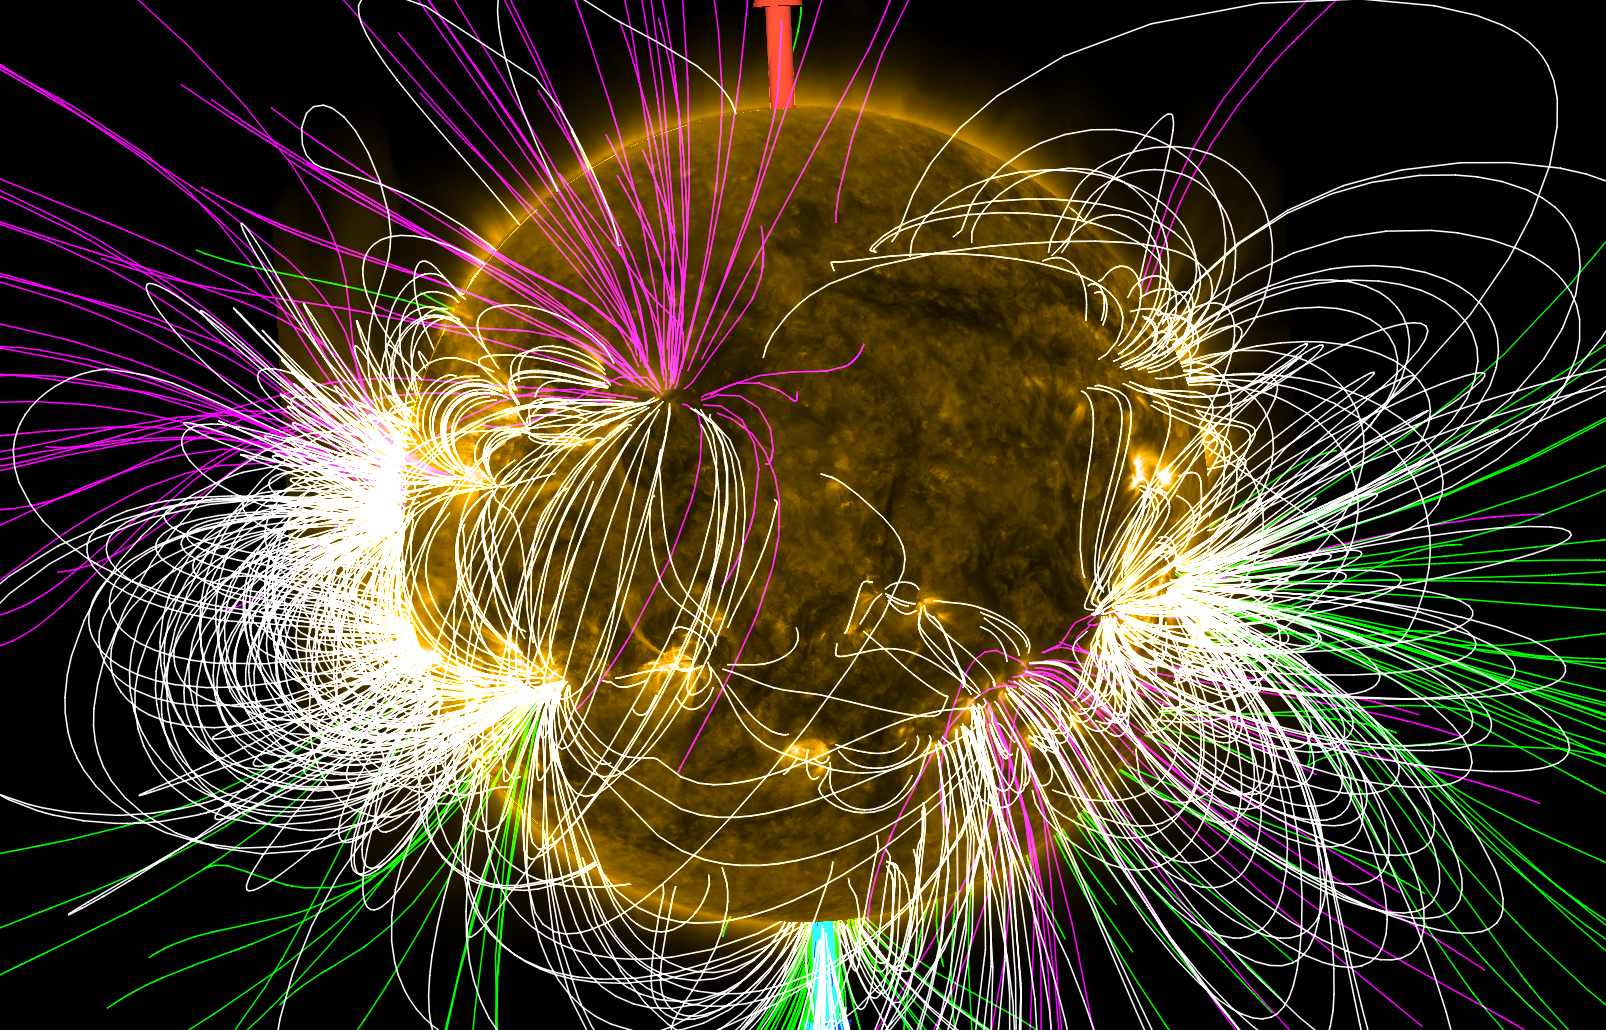
\includegraphics[width=0.8\textwidth,height=8cm,keepaspectratio]{./pictures/einleitung/fieldLines.png}
	\caption{Visualisierung der Feldlinien im JHelioviewer}
	\label{einleitung::feldlinien}
\end{figure}
Es wird zwischen drei Feldlinien Unterschieden: Linien, die auf der Sonne starten und wieder auf der Sonne landen, auf der Sonne starten und ins Weltall führen oder vom Weltall auf der Sonne landen. Die weissen Feldlinien repräsentieren ''Sonne zu Sonne´´, die Grünen ''Sonne zu Weltall´´ und die Violetten ''Weltall zu Sonne´´. Die Feldlinien sind, allgemein Betrachtet, eine grosse Menge an Punkten, welche ein Server bereitstellt. Die Abbildung \ref{einleitung::aufbau} visualisiert den Datenfluss.
\begin{figure}[!htbp]
\center
	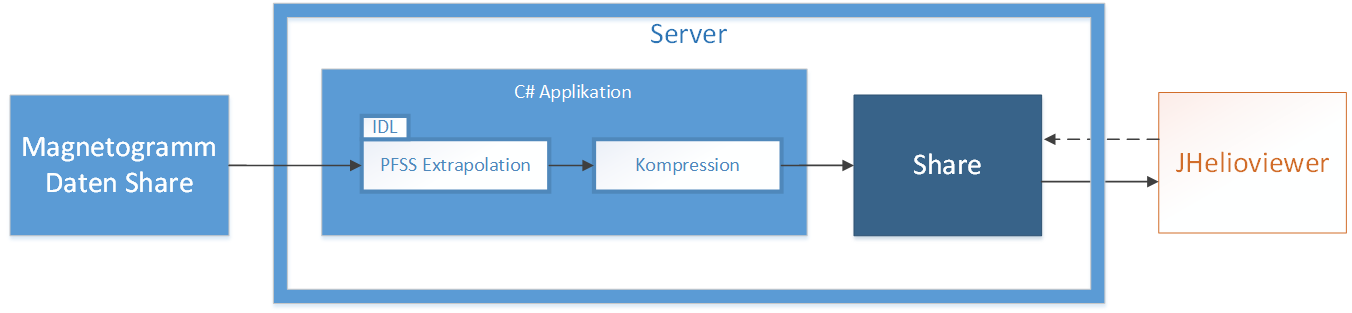
\includegraphics[width=0.8\textwidth,height=6cm,keepaspectratio]{./pictures/einleitung/server.png}
	\caption{Aufbau und Datenfluss des Servers}
	\label{einleitung::aufbau}
\end{figure}
In regelmässigen Abständen sucht der Server nach neuen Oberflächen-Magnetogramm-Daten der Satelliten. Die momentane Lösung erhält alle sechs Stunden neue Messdaten der Satelliten. Daraus werden mittels Potential Field Source Surface (PFSS) Simulation die Feldlinien zu diesem Zeitpunkt errechnet. Danach führt der Server eine Kompression durch und stellt die Daten auf einem öffentlichen Share dem JHelioviewer zur Verfügung. Zusammen mit Aufnahmen von anderen Instrumenten animiert der JHelioviewer die Feldlinien über einen gewissen Zeitraum. Die Daten werden zur Laufzeit über eine Internetverbindung nachgeladen.

\subsection{Rohdatenmenge der Feldlinien}
Die PFSS Extrapolation produziert für eine Aufnahme etwa 15 MiBytes an Daten.
Verlustfrei/verlustbehaftet.
Vorfeld schon mit Verlustlosen und Verlustbehafteten Kompressionsverfahren auf etwa 1.5 MiByte verkleinert.
Ziel ist es, so wenige Daten wie Möglich zu brauchen. Zukunftsvision




 